\documentclass[10pt]{article}
\usepackage{parskip}
\usepackage[utf8]{inputenc}
\usepackage[left=2.00cm, right=2.00cm, top=2.00cm, bottom=2.00cm]{geometry}
\usepackage[spanish]{babel}
\usepackage{graphicx,subfig}
\usepackage{fancyhdr}
\graphicspath{{Imagenes/}}
\usepackage{enumerate} 
\usepackage{multicol}
\begin{document}


\pagestyle{fancy}
\cfoot{}


%Cabeceras
\rhead{Conocimiento y manejo del Osciloscopio}
\lhead{}

%Portada
\begin{titlepage}
	\newgeometry{
		left=25mm,
		right=25mm,
		top=5mm,
		bottom=30mm,
		headheight = 0 mm
	}

	\begin{figure}[t]
		\subfloat{
\includegraphics[width=0.15\textwidth]{Logo_IPN}}
		\hspace{0.7\textwidth}
		\subfloat{
\includegraphics[width=0.22\textwidth]{LogoEsime}}
	\end{figure}

	\centering
	{\bfseries\Huge Instituto Politécnico Nacional. \par}
	\vspace{1cm}
	{\scshape\Large Ingeniería en Comunicaciones y Electrónica. \par}
	\vspace{0.3cm}
	{\scshape\Large Laboratorio de Electricidad y Magnetismo.  \par}
	\vspace{1cm}
	{\scshape\Huge LAS ONDAS \par}
	\vspace{1cm}
	{\itshape\Large Conocimiento y manejo del Osciloscopio. \par}
	{\Large 2CM13\par}
	\vfill
	{\Large Autores: \par}
	{\Large Daniela Elizabeth Pérez Vargas. \par}
	{\Large Jesús Martinez Amac. \par}
	{\Large José Emilio Hernández Huerta. \par}
	{\Large Nataly Bejarano Garduño..\par}
	{\Large Uriel Grimaldi Díaz.  \par}
	\vfill
	{\Large Abril 2023. \par}

\end{titlepage}

\tableofcontents
\newpage




\section{Resumen.}
Por medio de instrumentos especializados se observo el comportamiento de multiples funciones de onda por medio de un osciloscopio el cual muestra en pantalla de una forma grafica al igual que se aprendera a utilizar un generador de funciones de onda para mostrarlas en la pantalla del osciloscopio.

\begin{multicols}{2}
\section{Objetivo.}
El alumno identificara las perillas y botones requeridos para un empleo básico del osciloscopio, calibrara el osciloscopio en frecuencia y voltaje, efectuara la medicion de tensiones directas y alternas y por ultimo realizara la medicion de la frecuencia y periodo de una señal.

\section{Introducción.}
Las funciones de ondas nos ayudan a comprender de mejor forma los comportamientos de algunos sistemas un ejemplo de esto seria en la reparacion de un celular al poder medir el consumo de energia con respecto al tiempo nos proporciona informarcion util como; porque no llega a prender, componentes dañados, corto circuitos, ect. También es de gran ayuda para poder estudiar de mejor forma el campo de la electricidad. Por eso es importante que el estudiante aprenda a manejar de forma correcta un osciloscopio.


\section{Marco teórico.}
El Generador de señales: Un Generador de Señales es un instrumento de laboratorio que permite crear electrónicamente diferentes tipos de señales a diferentes frecuencias y diferentes amplitudes.
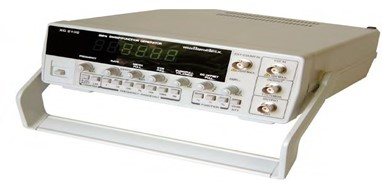
\includegraphics[width=0.1\textwidth]{Imagenes/Marco Teorico/Imagen1}
Señal Sinusoidal
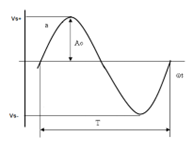
\includegraphics[width=0.1\textwidth]{Imagenes/Marco Teorico/Imagen2}
Señal Triangular
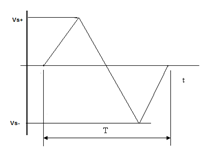
\includegraphics[width=0.1\textwidth]{Imagenes/Marco Teorico/Imagen3}
Señal Cuadrada
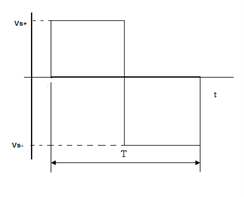
\includegraphics[width=0.1\textwidth]{Imagenes/Marco Teorico/Imagen4}
En donde:
T = Periodo de la señal. 
Vs+ = Voltaje positivo Máximo
Vs- = Voltaje negativo Máximo
A0 = Amplitud de la señal.
Es importante recordar que la frecuencia de la señal (en Hz) está dada por:
F= 1/T
Y que el Voltaje Pico a Pico o Vpp está dado por:
$Vpp= (Vs+) – (Vs-)$
Los generadores de señales tienen un rango de frecuencia y amplitudes de funcionamiento y permiten entre otras funciones, calibración de equipos, pruebas a sistemas de audio, pruebas a servo motores.
El Osciloscopio es un aparato de medición que es capaz de mostrar señales eléctricas variantes en el tiempo. Además de la observación de estas señales con el osciloscopio es posible realizar análisis de frecuencia de la señal, determinar transitorios o cambios dinámicos en una señal.
Un osciloscopio esta constituido básicamente en los siguientes subsistemas.
1.- Tubo de rayos catódicos (CRT)
2.- Amplificadores verticales y horizontales
3.- Circuito Base de tiempo
4.-Fuentes de potencia
El osciloscopio es un equipo que sirve para visualizar formas de onda de TENSIÓN de un circuito. Las formas de onda las representan en dos ejes: el eje de abscisas representa tiempo y el eje de ordenadas representa tensión.

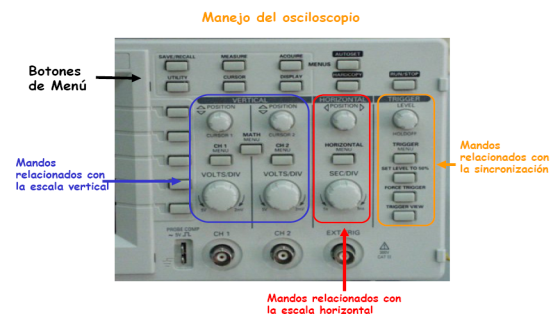
\includegraphics[width=0.1\textwidth]{Imagenes/Marco Teorico/Imagen5 pero usa el tuyo .png}
Las escalas de ambos ejes son modificables por el usuario. La pantalla está dividida en cuadrículas y lo que el usuario elige es el valor de cada una de esas cuadrículas.
Ejemplo de la pantalla del osciloscopio:
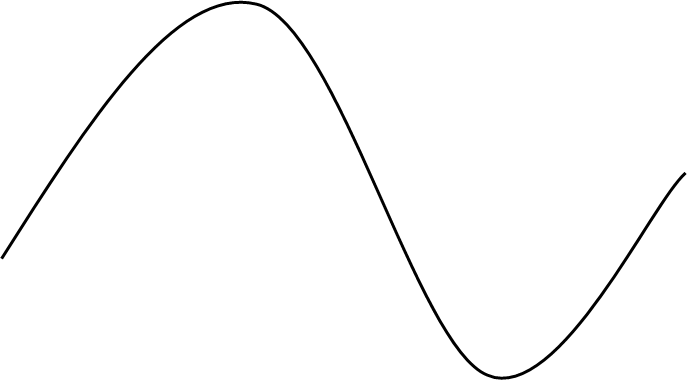
\includegraphics[width=0.1\textwidth]{Imagenes/Marco Teorico/Imagen6}
Cada línea horizontal representa un voltaje que puede ser variado con las perillas del osciloscopio ( Volts / Division)
Cada línea Horizontal representa una escala de tiempo que puede ser variada con la perilla del osciloscopio ( Time/ Division)




\section{Descripción de materiales.}

 

\section{Desarrollo experimental.}





\section{Análisis y resultados.}




\section{Discución.}

\section{Conclusiones.}
\subsection{José Emilio Hernández Huerta}

\subsection{Jesus Martinez Amac}

\subsection{Nataly Garduño Bejarano}


\subsection{Perez Vargas Daniela Elizabeth}


\end{multicols}
\newpage
\clearpage
\begin{thebibliography}{0}
	\bibitem{}[Escamilla, E.(2017).Distribución de cargas eléctricas en los conductores.]
	www.academia.edu.
\end{thebibliography}

\end{document}

